%%
%% This is file `sample-sigconf.tex',
%% generated with the docstrip utility.
%%
%% The original source files were:
%%
%% samples.dtx  (with options: `sigconf')
%% 
%% IMPORTANT NOTICE:
%% 
%% For the copyright see the source file.
%% 
%% Any modified versions of this file must be renamed
%% with new filenames distinct from sample-sigconf.tex.
%% 
%% For distribution of the original source see the terms
%% for copying and modification in the file samples.dtx.
%% 
%% This generated file may be distributed as long as the
%% original source files, as listed above, are part of the
%% same distribution. (The sources need not necessarily be
%% in the same archive or directory.)
%%
%%
%% Commands for TeXCount
%TC:macro \cite [option:text,text]
%TC:macro \citep [option:text,text]
%TC:macro \citet [option:text,text]
%TC:envir table 0 1
%TC:envir table* 0 1
%TC:envir tabular [ignore] word
%TC:envir displaymath 0 word
%TC:envir math 0 word
%TC:envir comment 0 0
%%
%%
%% The first command in your LaTeX source must be the \documentclass
%% command.
%%
%% For submission and review of your manuscript please change the
%% command to \documentclass[manuscript, screen, review]{acmart}.
%%
%% When submitting camera ready or to TAPS, please change the command
%% to \documentclass[sigconf]{acmart} or whichever template is required
%% for your publication.
%%
%%
\documentclass[sigconf]{acmart}
% \documentclass[sigconf, manuscript]{acmart} %单栏

%%
%% \BibTeX command to typeset BibTeX logo in the docs
\AtBeginDocument{%
  \providecommand\BibTeX{{%
    Bib\TeX}}}

%% Rights management information.  This information is sent to you
%% when you complete the rights form.  These commands have SAMPLE
%% values in them; it is your responsibility as an author to replace
%% the commands and values with those provided to you when you
%% complete the rights form.

% \setcopyright{acmlicensed}
% \copyrightyear{2024}
% \acmYear{2024}
% \acmDOI{XXXXXXX.XXXXXXX}

%% These commands are for a PROCEEDINGS abstract or paper.
% \acmConference[BDDM '24]{The 2nd International Conference on Big Data and Data Mining}{December 14, 2024}{Wuhan, China}
%%
%%  Uncomment \acmBooktitle if the title of the proceedings is different
%%  from ``Proceedings of ...''!
%%
%%\acmBooktitle{Woodstock '18: ACM Symposium on Neural Gaze Detection,
%%  June 03--05, 2018, Woodstock, NY}

% \acmISBN{978-1-4503-XXXX-X/18/06}

\renewcommand\footnotetextcopyrightpermission[1]{} %移除页脚的说明
\settopmatter{printacmref=false} %remove ACM reference format

%%
%% Submission ID.
%% Use this when submitting an article to a sponsored event. You'll
%% receive a unique submission ID from the organizers
%% of the event, and this ID should be used as the parameter to this command.
%%\acmSubmissionID{123-A56-BU3}

%%
%% For managing citations, it is recommended to use bibliography
%% files in BibTeX format.
%%
%% You can then either use BibTeX with the ACM-Reference-Format style,
%% or BibLaTeX with the acmnumeric or acmauthoryear sytles, that include
%% support for advanced citation of software artefact from the
%% biblatex-software package, also separately available on CTAN.
%%
%% Look at the sample-*-biblatex.tex files for templates showcasing
%% the biblatex styles.
%%

%%
%% The majority of ACM publications use numbered citations and
%% references.  The command \citestyle{authoryear} switches to the
%% "author year" style.
%%
%% If you are preparing content for an event
%% sponsored by ACM SIGGRAPH, you must use the "author year" style of
%% citations and references.
%% Uncommenting
%% the next command will enable that style.
%%\citestyle{acmauthoryear}


%%
%% end of the preamble, start of the body of the document source.

% correct bad hyphenation here
\hyphenation{op-tical net-works semi-conduc-tor}

% \usepackage{cite} %不要打开,会与参考文献冲突,导致不显示
\usepackage{amsmath,amssymb,amsfonts}
\usepackage{algorithmic}
\usepackage{graphicx}
\usepackage{textcomp}
\usepackage{xcolor}

%新增定义
\usepackage[ruled,vlined]{algorithm2e}
\usepackage{amsthm}
\usepackage{array} % 用于自定义列对齐
\usepackage{booktabs} % 用于生成更美观的表格线
\usepackage{graphicx} % 用于 \resizebox 命令
\usepackage{url}
%
%
\newtheorem{definition}{Definition}
\newtheorem{example}{Example}

\copyrightyear{2024}
\acmYear{2024}
\setcopyright{rightsretained}
\acmConference[CIoTSC 2024]{2024 2nd International Conference on Computer, Internet of Things and Smart City}{December 27--29, 2024}{Nanchang, China}
\acmBooktitle{2024 2nd International Conference on Computer, Internet of Things and Smart City (CIoTSC 2024), December 27--29, 2024, Nanchang, China}
\acmPrice{}
\acmDOI{10.1145/3731867.3731898}
\acmISBN{979-8-4007-1472-6/24/12}

\begin{document}

%%
%% The "title" command has an optional parameter,
%% allowing the author to define a "short title" to be used in page headers.
\title{Landmark Selection Strategy to Accelerate Shortest Distance Queries}

%%
%% The "author" command and its associated commands are used to define
%% the authors and their affiliations.
%% Of note is the shared affiliation of the first two authors, and the
%% "authornote" and "authornotemark" commands
%% used to denote shared contribution to the research.

\author{Zhipeng He}
\orcid{0009-0006-8888-5975}
\email{2112233062@e.gzhu.edu.cn}
\affiliation{%
  \institution{Guangzhou University}
  \city{Guangzhou}
  \country{China}
}

\author{Dian Ouyang}
\authornote{Corresponding author.}
\orcid{0000-0002-9472-4389}
\email{dian.ouyang@gzhu.edu.cn}
\affiliation{%
  \institution{Guangzhou University}
  \city{Guangzhou}
  \country{China}
}

\author{Jianye Yang}
\orcid{0000-0003-3417-823X}
\email{jyyang@gzhu.edu.cn}
\affiliation{%
  \institution{Guangzhou University}
  \city{Guangzhou}
  \country{China}
}

\renewcommand{\shortauthors}{Z. He, D. Ouyang, J. Yang}
%%
%% By default, the full list of authors will be used in the page
%% headers. Often, this list is too long, and will overlap
%% other information printed in the page headers. This command allows
%% the author to define a more concise list
%% of authors' names for this purpose.

%%
%% The abstract is a short summary of the work to be presented in the
%% article.
\begin{abstract}
Computing the shortest path between vertices is a fundamental task in network analysis. This paper introduces an innovative strategy for selecting landmarks in a graph, which improves upon the traditional highest-degree selection method. Our approach captures the essential structural features of graphs, effectively reducing landmark overlap and clustering. Combined with partition querying and upper-bound pruning optimizations, our algorithm achieves a notable $20 \%-30 \%$ increase in query speed and is applicable to multi-million record datasets. This study offers new insights and solutions for enhancing query performance in large-scale graph-structured data, paving the way for further innovations in graph database optimization to meet the growing demands of large-scale graph data processing.\par

\end{abstract}

%%
%% The code below is generated by the tool at http://dl.acm.org/ccs.cfm.
%% Please copy and paste the code instead of the example below.
%%
\begin{CCSXML}
<ccs2012>
   <concept>
       <concept_id>10003752.10003809.10003635</concept_id>
       <concept_desc>Theory of computation~Graph algorithms analysis</concept_desc>
       <concept_significance>500</concept_significance>
       </concept>
 </ccs2012>
\end{CCSXML}

\ccsdesc[500]{Theory of computation~Graph algorithms analysis}


\keywords{Shortest path, landmark, distance labeling, optimization}

%%
%% This command processes the author and affiliation and title
%% information and builds the first part of the formatted document.
\maketitle

\section{Introduction}
% no \IEEEPARstart
Finding the shortest path is a core problem in data mining and network analysis when dealing with large-scale graph data, with a wide range of applications including but not limited to traffic planning, social network analysis, and network routing optimization\cite{ref11}. With the continuous growth of data scale, traditional shortest path algorithms face enormous challenges in terms of efficiency and scalability. How to quickly and accurately calculate the shortest path has become an urgent problem that needs to be solved.\par
Current state-of-the-art algorithms in shortest path computations leverage landmark labeling-based approaches, which typically require specifying a parameter `K' to denote the number of landmarks \cite{ref6, ref7}. These algorithms conventionally select the top `K' vertices with the highest degree values within the graph to serve as landmarks.\par
%
\subsection{Motivation}
We believe that there is still optimization space by using only the top $k$ vertices with the highest degree as landmarks. To try different strategies, we considered using the top $k$ vertices with the highest betweenness centrality as the landmark. However, although there has been some improvement in label size, it has not shown significant improvement in actual queries. More importantly, due to the high time-consuming burden of calculating betweenness centrality in large graphs, we have to abandon this method. By analyzing the strategy of directly using vertices with the highest degree and betweenness centrality as landmarks \cite{ref6, ref7, ref8}, we found two main issues: firstly, the landmarks selected based on betweenness centrality overlap with those selected by the degree, and this situation is particularly prominent in large networks. Secondly, in highly clustered networks, strong clustering phenomena may lead to a core–periphery structure \cite{ref4, ref17}, resulting in relatively clustered selected vertices that we expect to be more dispersed in order to better cover the entire graph. Therefore, we are trying to find new algorithmic inspirations.


\subsection{Our idea}
We propose a novel landmark selection strategy: (1) Firstly, we use the Top-k degree vertices as benchmark landmarks and assign other vertices to the region where their nearest landmarks are located. (2) Next, within each region, we further select the vertex with the highest degree as the new landmark. This process aims to address vertex overlap and clustering issues, thereby improving query efficiency. It should be emphasized that in the selection of new landmarks, we only focus on the vertices with the highest degree within each region, without considering vertices across regions. This detail ensures that the new landmarks can be scattered throughout the entire graph and not clustered in a specific local area. (3) During the query phase, we further introduced optimization for partitioned queries.

\subsection{Contribution}
In this paper, our main contributions are as follows: \par
\begin{itemize}
\item An innovative landmark selection strategy in the graph has been proposed, which can better capture important features of the graph structure and effectively reduce the overlap and clustering phenomena between landmarks compared to the traditional highest degree selection method.\par
\item The concept of region partitioning has been introduced, assigning vertices to the regions where their nearest landmarks are located, resulting in a more dispersed distribution of landmarks throughout the entire graph, reducing clustering and improving query efficiency.\par
\item The proposed landmark selection strategy and query optimization method have good scalability and universality, and are suitable for various practical application scenarios such as graph databases and social networks. Even when processing billion level datasets, they can perform well, providing strong support for research and applications in related fields.\par
\end{itemize}
%
%
\subsection{Outline}

The paper is structured as follows. In Section \ref{sec:Preliminary}, we introduce the problem definitions and preliminary. We briefly describe the existing solutions in Section \ref{sec:existing_solutions}. In Section \ref{sec:Framework}, we introduce the Distance Query Framework, while Section \ref{sec:landmark_selection} is dedicated to optimizing the landmark selection strategy. Section \ref{sec:Experiment} presents experiments that evaluate our methods. Finally, Section \ref{sec:conclusion} concludes this paper.\par
%
%
\section{Preliminary}
\label{sec:Preliminary}
Let $G=(V,E)$ be a graph, where $V$ is the set of vertices and $E$ is the set of edges. We denote the number of vertices and edges by $n = |V|$ and $m = |E|$, respectively. For simplicity, we assume that the $G$ is connected and undirected throughout this paper, since our work can be easily extended to directed or disconnected graphs. Let $G[V\setminus R]$ represent removing all landmarks set in $R$ from $G$, and $d_{G}(s,t)$ represent the shortest distance from $s$ to $t$.\par

\subsection{Distance labeling}
Let $R \subseteq V$ be a set of special vertices in $G$, called landmarks, a label $L(v)$ for each vertex $v \in V$ can be precomputed, which can be answered in linear-time by looking up the label $L(v)$. The collection of labels $L=\{L(v)\}_{v \in V}$ is referred to as a distance labeling on graph $G$. The distance between two vertices $s$ and $t$ can be calculated as:\par

\begin{center}
$\operatorname{d}_{G}(s, t)=\min _{r \in L(s) \cap L(t)} \left ( \operatorname{d}_{G}(s, r)+\operatorname{d}_G(r, t) \right )$
\end{center}
%
% figure1
%
\begin{figure}
\centering
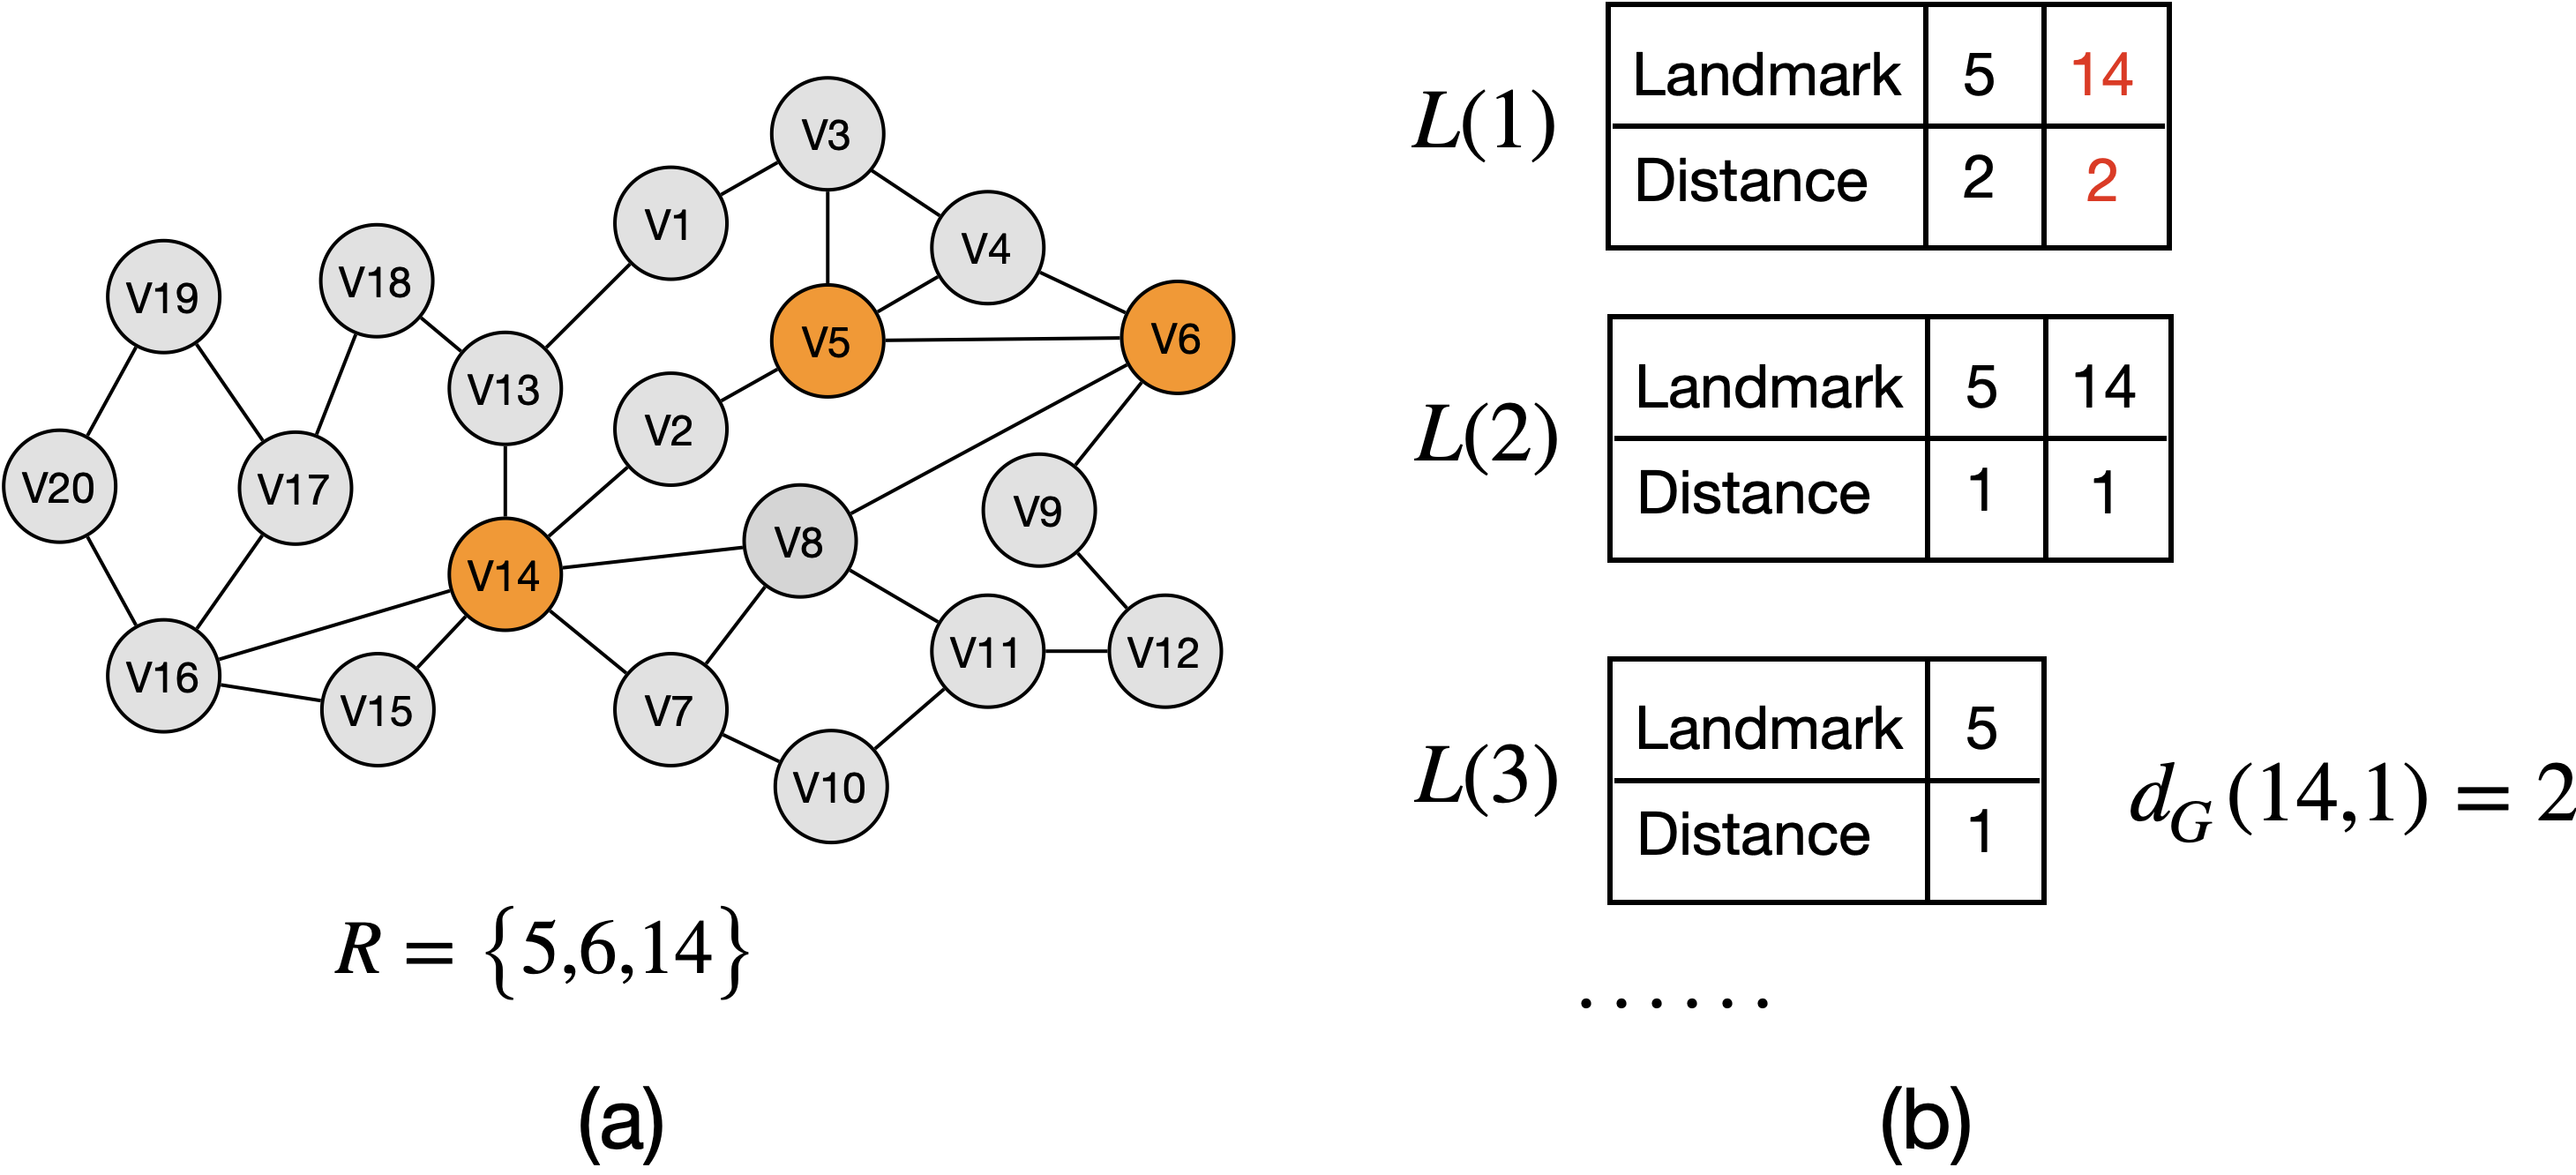
\includegraphics[width=0.45\textwidth]{figures/2-1-distance-labeling.png}
\caption{An explanation of distance labeling:(a) an example graph G, (b) Compute a label $L\left ( v \right ) $ for each vertex $v\in V$ in $G$ in advance.} \label{fig1}
\end{figure}

%
% example1
%
\begin{example}
    Consider the graph $G$ depicted in Fig.1(a), with a set of landmarks $R=\left \{ 5,6,14 \right \} $ and precomputed distance labels $L(1)=\{(5,2),(14,2)\}$, $L(2)=\{(5,1),(14,1)\}$ and $L(3)=\{(5,1)\}$, etc. in Fig.1(b), we can efficiently determine that $d_{G}(14,1)=2$.
\end{example}

\subsection{Problem Definition}
Given a graph $G$ and a set of precomputed landmarks $R \subseteq V$, a shortest distance query $q =(s, t)$ is defined, where $s, t \in V$, and the answer is the shortest distance $d_{G}(s, t)$. This paper aims to develop efficient landmark selection strategies to optimize query performance. Specifically, our objective is to minimize the total query time, $T(Q)=min {\textstyle \sum_{q\in Q}T(q,R)} $ where $T(q,R)$ represents the time taken to answer the query $q$ using the set of landmarks $R$.\par

%
% example2
%
\begin{example}
    Fig.1(a) shows a network $G=(V,E)$ with 20 vertices and 30 edges. There are many paths between $v_{12}$ and $v_{19}$. For example, two of them are $p_{1}=\left(v_{12}, v_{11}, v_{8}, v_{14}, v_{13}, v_{18},v_{17},v_{19})\right.$ and $p_{2}=\left(v_{12}, v_{9}, v_{6}, v_{5}, v_{2}, v_{14}, v_{16}, v_{20}, v_{19}\right)$ with $d_{G}(p_{1})= 7$ and $d_{G}(p_{2})=8$. $p_{1}$ is a shortest path between $v_{12}$ and $v_{19}$ as covered by landmark $v_{14}$. Given a shortest distance query $q=\left(v_{12}, v_{19}\right)$, the answer of $q$ is $d(v_{12}, v_{19})=7$.
\end{example}
%
%
\section{Existing Solutions}
\label{sec:existing_solutions}
This section formalizes two distance labeling concepts: 2-hop labeling and Highway cover labeling\cite{ref1, ref7}, which lay the foundation for our theoretical analysis and new algorithm.\par

\subsection{2-Hop Labeling}
The 2-hop labeling technique is commonly used in methods for shortest path computation\cite{ref6, ref7, ref11, ref12, ref16}. Given a network $G$, 2-hop labeling assigns each vertex $v \in V$ a label $L(v)$ which is a collection of pairs $(u, \operatorname{d}_{G}(v, u))$ where $u \in V$. \par

\begin{definition}
    \textbf{(2-hop cover labeling)}. A labeling $L$ is a 2-hop Cover labeling of $G$ if, for each pair $s, t \in V$, $L(s) \cap L(t)$ contains at least one common vertex $r$ on the shortest path from $s$ to $t$. This guarantees that:\par
    \begin{center}
        $Query_(s, t, L) = \min \{ \delta_L(r, s) + \delta_L(r, t) \mid r \in L(s) \cap L(t) \}$
    \end{center}
\end{definition}
Thus, we determine $d_G(s, t)$ by scanning both $L(s)$ and $L(t)$, with a query time complexity of $O(|L(s)| + |L(t)|)$.

%
%
\subsection{Highway Cover Labeling}
We start by providing the definitions of highway and highway cover labeling scheme \cite{ref7, ref10}.

\begin{definition}
    \textbf{(Highway)}. A highway $H$ can be defined as a tuple $\left(R, \delta_{H}\right)$ consists of a distance decoding function $\delta_{H}$ and a set $R$ of landmarks, the value $\delta_{H}$ corresponds to the shortest path distance $d_{G}\left(r_{1}, r_{2}\right)$, i.e.
  $\delta_{H}\left(r_{1}, r_{2}\right)=d_{G}\left(r_{1}, r_{2}\right)$.\par
\end{definition}
%
%
\begin{figure}
\centering
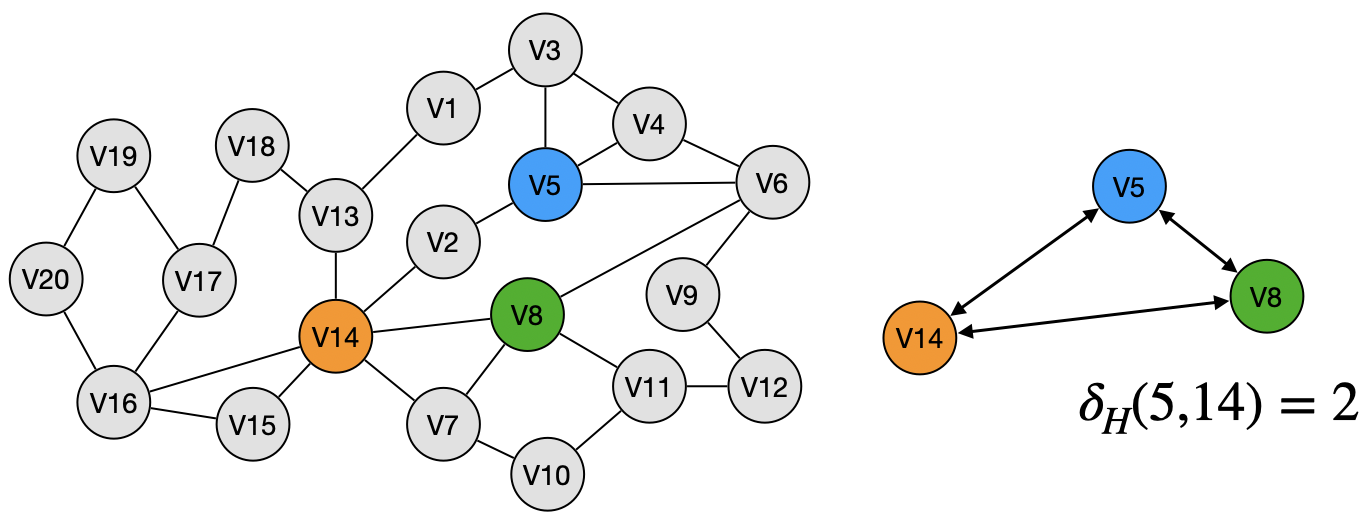
\includegraphics[width=0.45\textwidth]{figures/3-1-highway.png}
\caption{Highway Labeling} \label{fig2}
\end{figure}

\begin{example}
    Refer to the graph $G$ shown in the Fig.~\ref{fig2}, we select the set $R=\{5,8,14\}$ as landmarks. The distance decoding function $\delta_{H}$ is specified as follows: $\delta_{H}(5,14)$ denotes the shortest path distance from vertices 5 to 14, which is 2. Similarly, $\delta_{H}(5,8)$ is 2 and  $\delta_{H}(8,14)$ is 1.
\end{example}
%    
%
 This highway $H$ effectively represents the landmark distance relationships within graph $G$, facilitating the rapid computation or estimation of shortest paths between vertices.

\begin{definition}
    \textbf{(Highway Cover Labeling)}. A highway cover labelling $\Gamma=(H, L)$ consists of a highway $H$ and a distance labeling $L$. Then for any vertices $u \in V \backslash R$ and for any $r \in R$, there exist $r^{\prime} \in R$ in $L(u)$ such that $r^{\prime}$ lies on the shortest path from $u$ to $r$ \text {(} where $r$ \text {and} $r^{\prime}$ \text {may be the same). }
\end{definition}

%
% figure3
%
\begin{figure}
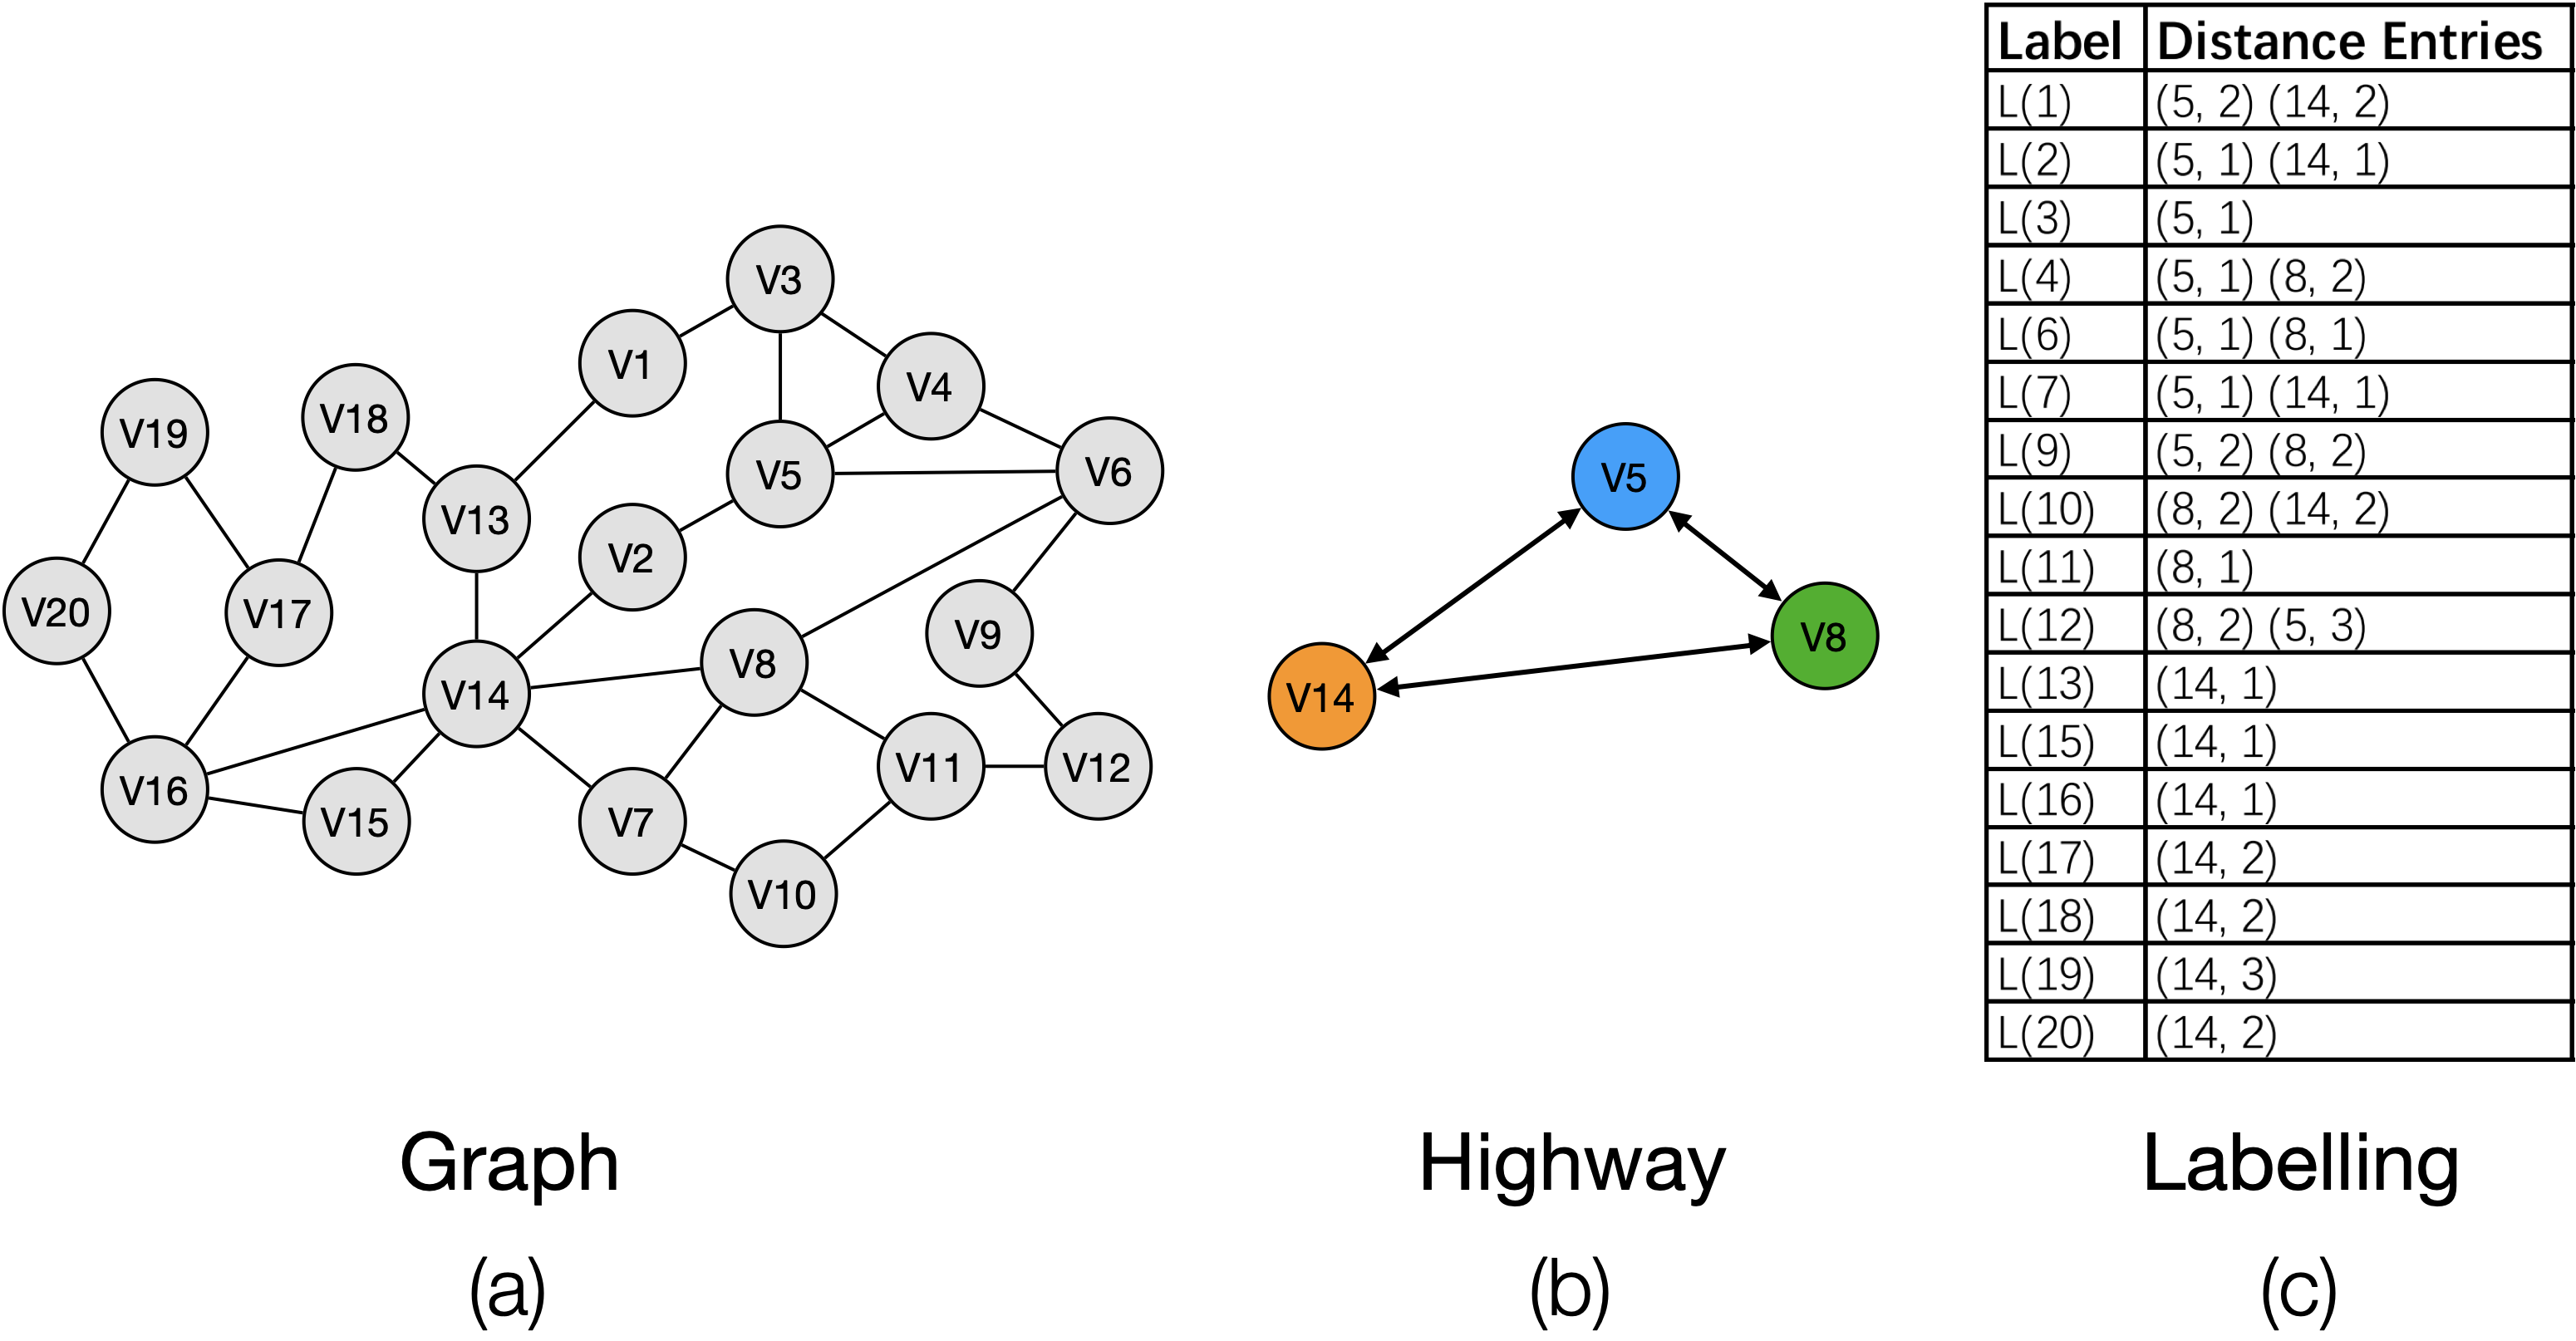
\includegraphics[width=0.45\textwidth]{figures/3-2-highway-cover.png}
\caption{Highway Cover Labeling} \label{fig3}
\end{figure}
%

%
% example4
%
\begin{example}
    In the network illustrated in the Fig.~\ref{fig3}(a), the highway $H$ includes three landmarks: $5$, $8$, and $14$, highlighted in Fig.~\ref{fig3}(b). The path $p_{1}=\left(v_{3}, v_{5}, v_{4})\right.$ denotes the shortest path between vertices $3$ and $4$, which is constrained by landmark $5$. In contrast, neither of paths $p_{2}=\left(v_{3}, v_{1}, v_{13}, v_{14}, v_{2}, v_{5}, v_{4})\right.$ and $p_{3}=\left(v_{3}, v_{4})\right.$ satisfies the condition of being a shortest path between 3 and 4 constrained by landmark 5.\par
\end{example}

In contrast to a 2-hop cover labeling, a highway cover labeling can only answer distance queries between landmarks and other vertices in the graph, making it a partial distance labeling\cite{ref12}.\par

How to choose a better landmark set will be explained in detail in the section \ref{sec:landmark_selection}, which is the main part of our algorithm.
%
%
\section{Distance Query Framework}
\label{sec:Framework}
In this section, we present the distance query framework, which facilitates efficient and accurate batch computation of shortest distances for any pair of vertices in a large graph.

\subsection{Label Construction}
%
%
%【algorithm1】
%
\begin{algorithm}
\caption{Construct highway cover labeling $L$}
\KwIn{Network $G(V, E)$, Highway $H(R, \delta_H)$}
\KwOut{The highway cover labeling $L$}
$L(v) \gets \emptyset$ for all $v \in V \setminus R$\;
\ForEach{$r_i \in R$}{
    $Q_L \gets \emptyset$\;
    $Q_N \gets \emptyset$\;
    $Q_L.\text{push}(r_i)$\;
    $n \gets 0$\;
    
    \While{$Q_L$ and $Q_N$ are not empty}{
        \ForEach{$u \in Q_L$ at depth $n$}{
            \ForEach{$v \in \text{adj}[u]$}{
                \If{$v$ is unvisited}{
                    $\delta_{\text{BFS}}(r_i, v) \gets n + 1$\;
                    \eIf{$v$ is a landmark}{
                        $Q_N.\text{push}(v)$\;
                    }{
                        $Q_L.\text{push}(v)$\;
                        $L(v) \gets L(v) \cup \{(r_i, \delta_{\text{BFS}}(r_i, v))\}$\;
                    }
                }
            }
        }
        \ForEach{$u \in Q_N$ at depth $n$}{
            \ForEach{$v \in \text{adj}[u]$}{
                \If{$v$ is unvisited}{
                    $\delta_{\text{BFS}}(r_i, v) \gets n + 1$\;
                    $Q_N.\text{push}(v)$\;
                }
            }
        }
        $n \gets n + 1$\;
    }
}
\Return{$L$}
\end{algorithm}

%
% figure3
%
\begin{figure}
\centering
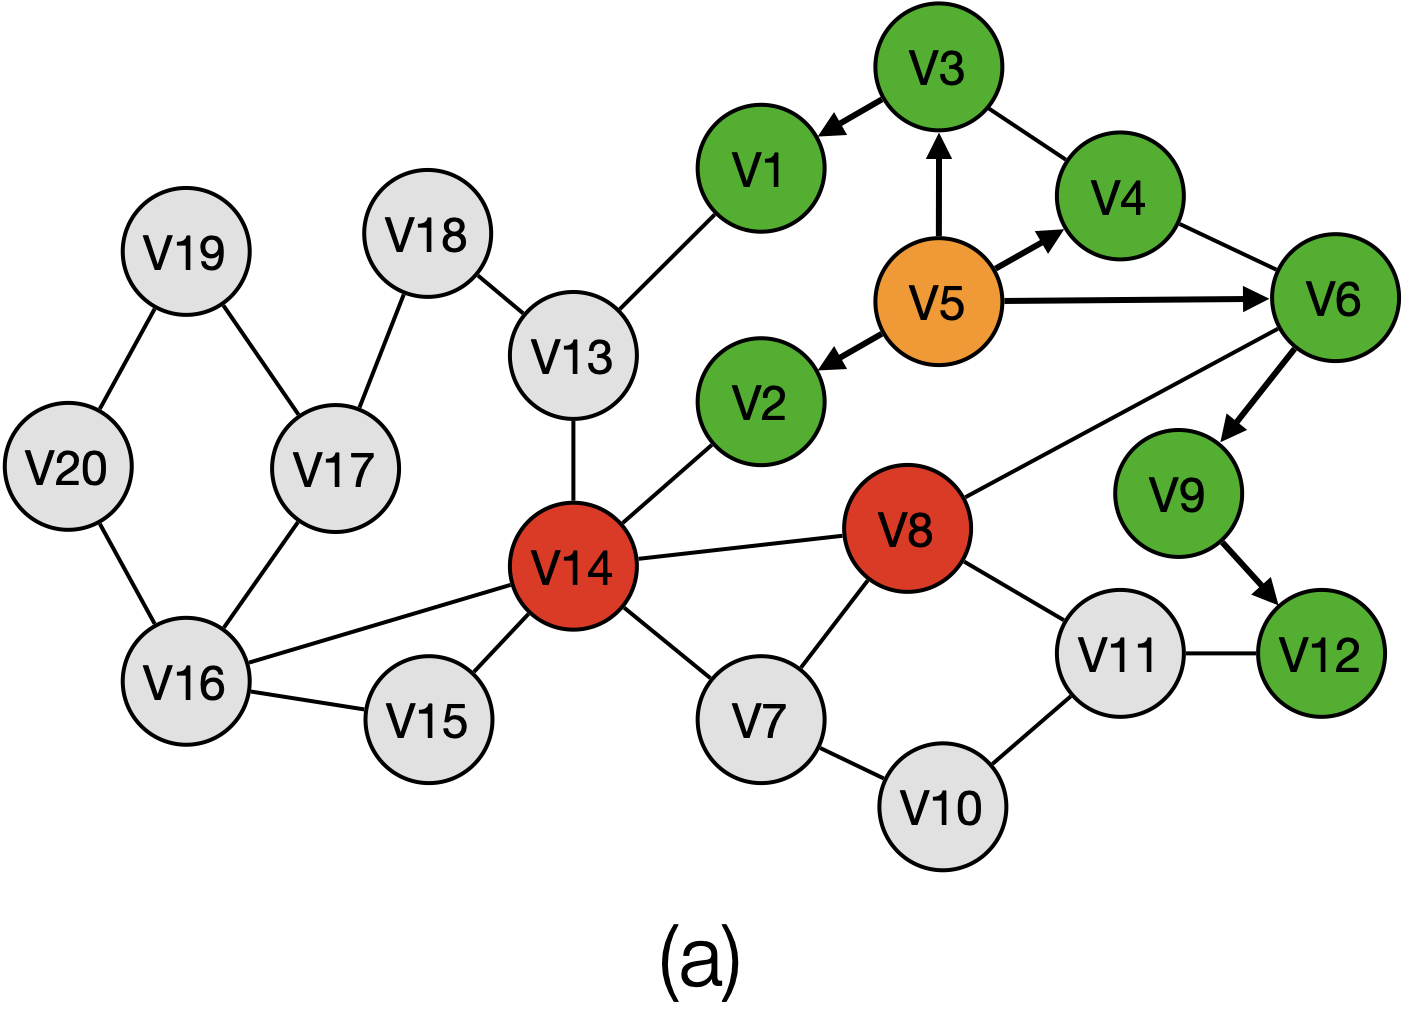
\includegraphics[width=0.3\textwidth]{figures/4-1-a-label-con.png} 
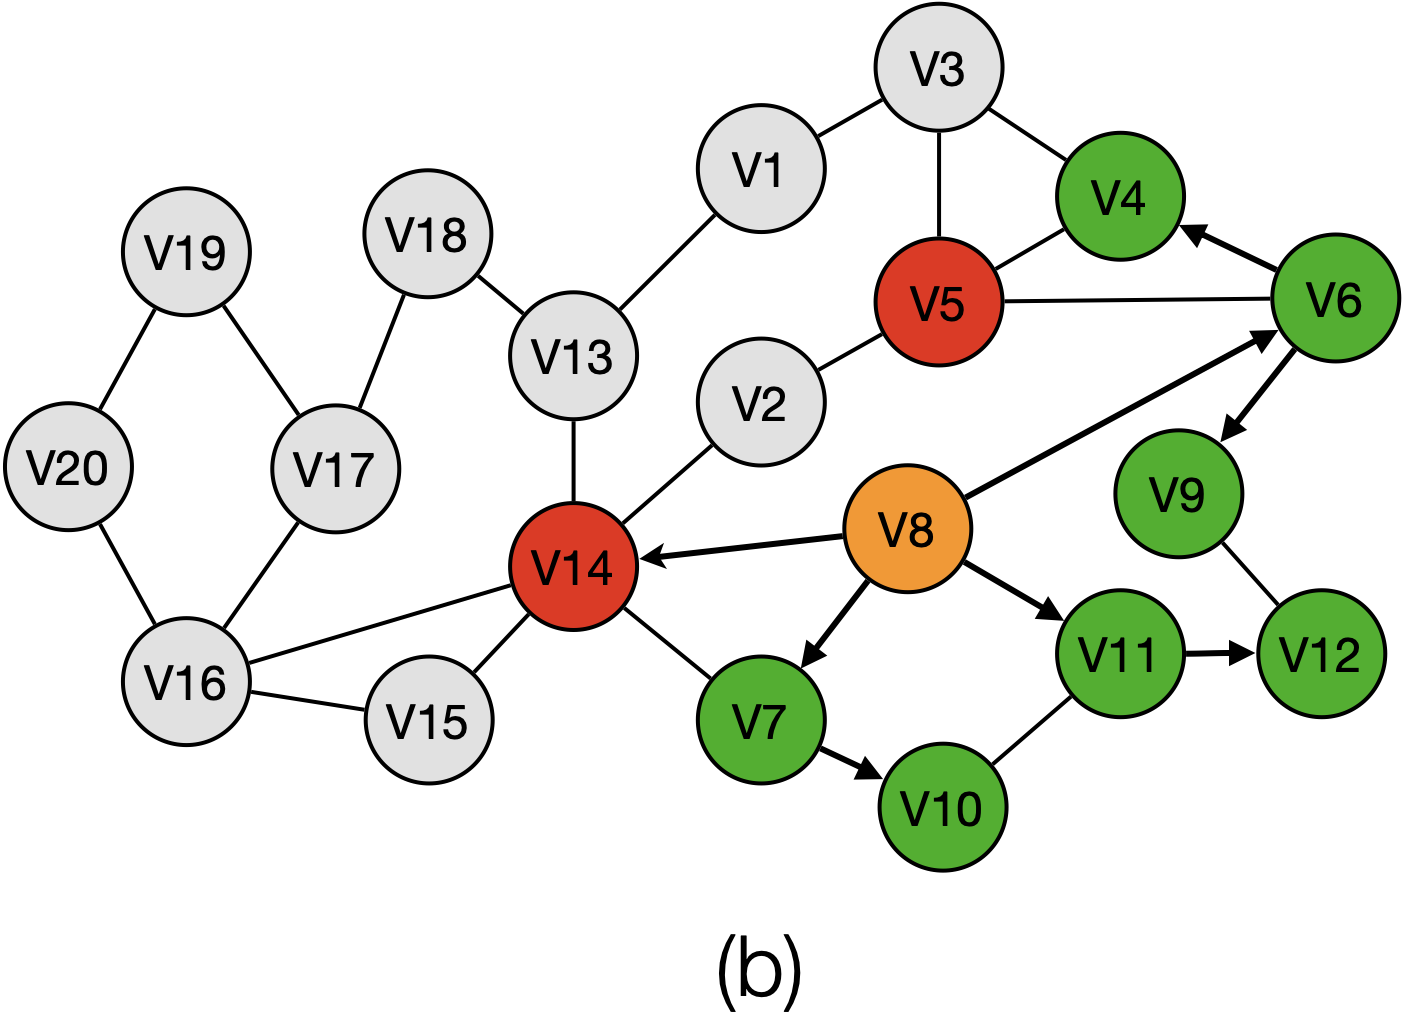
\includegraphics[width=0.3\textwidth]{figures/4-1-b-label-con.png}
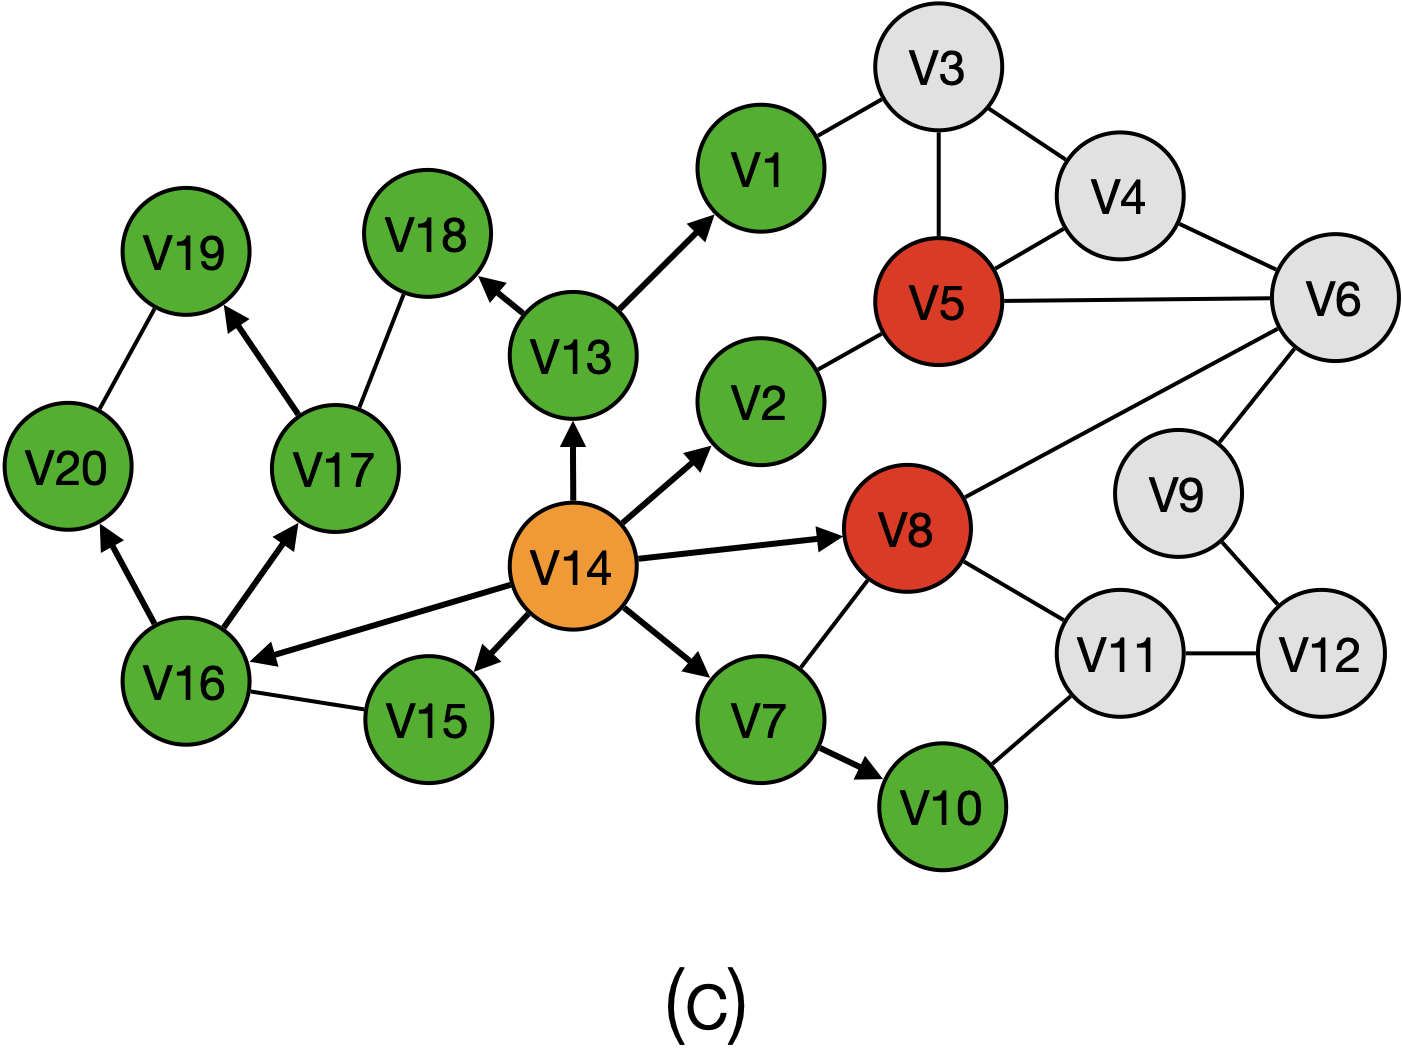
\includegraphics[width=0.3\textwidth]{figures/4-1-c-label-con.png}
\caption{Label Construction.} \label{fig4}
\end{figure}

The label construction in our algorithm is outlined in Algorithm 1. The procedure begins by performing a Breadth-First Search(BFS) from each landmark $r \in R$. During this process, a distance entry $(r, \delta(r, v))$ is added to the label of a vertex $v \in V \setminus R$ if no closer landmark $r' \in R$ lies on the shortest path from $r$ to $v$. This condition ensures that the label for $v$ reflects the shortest distance from the most proximal landmark, optimizing the search process in our graph queries. \par

In Fig.~\ref{fig4}, the green vertices are visited and stored, while the grey vertices are pruned and no stored. This is because when BFS traversal begins at landmark $r$, grey vertices are obstructed by other landmarks $r^{\prime}$.

\subsection{Query Distance}
\label{sec:query_distance}
 For any pair of vertices $s$ and $t$, a highway cover distance labeling scheme $L$ can be used to estimate an upper bound $\underline{d}_{s,t}$ for the shortest path distance from $s$ to $t$ can be determined as follows,
%
\begin{align}
\underline{d}_{s,t} &= distance[s][i] + distance[t][i] \tag{1} \\
\underline{d}_{s,t} &= distance[s][i] + highway[i][j] + distance[t][j] \tag{2}
\end{align}
\par
Here, Equation (1) represents the shortest distance from $s$ to $t$ passing through the landmark $r_{i}$. Equation (2) represents the shortest distance from s to t passing through both landmarks $r_{i}$ and $r_{j}$, where the distance between $r_{i}$ and $r_{j}$ can be directly obtained from the highway. \par
We conduct distance query as described in Algorithm 2. When $s$ and $t$ are in the same region, the upper bound is calculated using Equation (1). Conversely, when $s$ and $t$ are in different regions, the upper bound is computed using Equation (2). The next section we will provide a detailed explanation of how the regions are partitioned. \par

%
%【Algorithm2】
%
\begin{algorithm}
    \caption{Query Distance}
    \label{alg:query-distance}
    \KwIn{$s, t$}
    \KwOut{$d_{G}(s, t)$}
    \If{$vertexToRegion[s] == vertexToRegion[t]$}{
        Initialize queues and distances\;
        $dist\_upper \gets landmark\_distances[s][region] + landmark\_distances[t][region]$\;
        \While{both queues are not empty}{
            Select the smaller queue\;
            \While{selected queue is not empty}{
                \ForEach{$w$ in neighbors of current node}{
                    \If{$w$ already visited by other queue}{
                        \Return path length via $w$\;
                    }
                    Mark $w$ and push to queue\;
                }
            }
        }
        Reset and clear queues\;
        \Return $\min(res, dist\_upper)$\;
    }
    \Else{
        Initialize $m \gets 99$\;
        \ForEach{$i$ in $C[s]$}{
            \ForEach{$j$ in $C[t]$}{
                $m \gets \min(m, distances[s][i] + highway[vertices[s][i]][vertices[t][j]] + distances[t][j])$\;
            }
        }
        \Return $m$\;
    }
\end{algorithm}

\begin{figure}
\centering
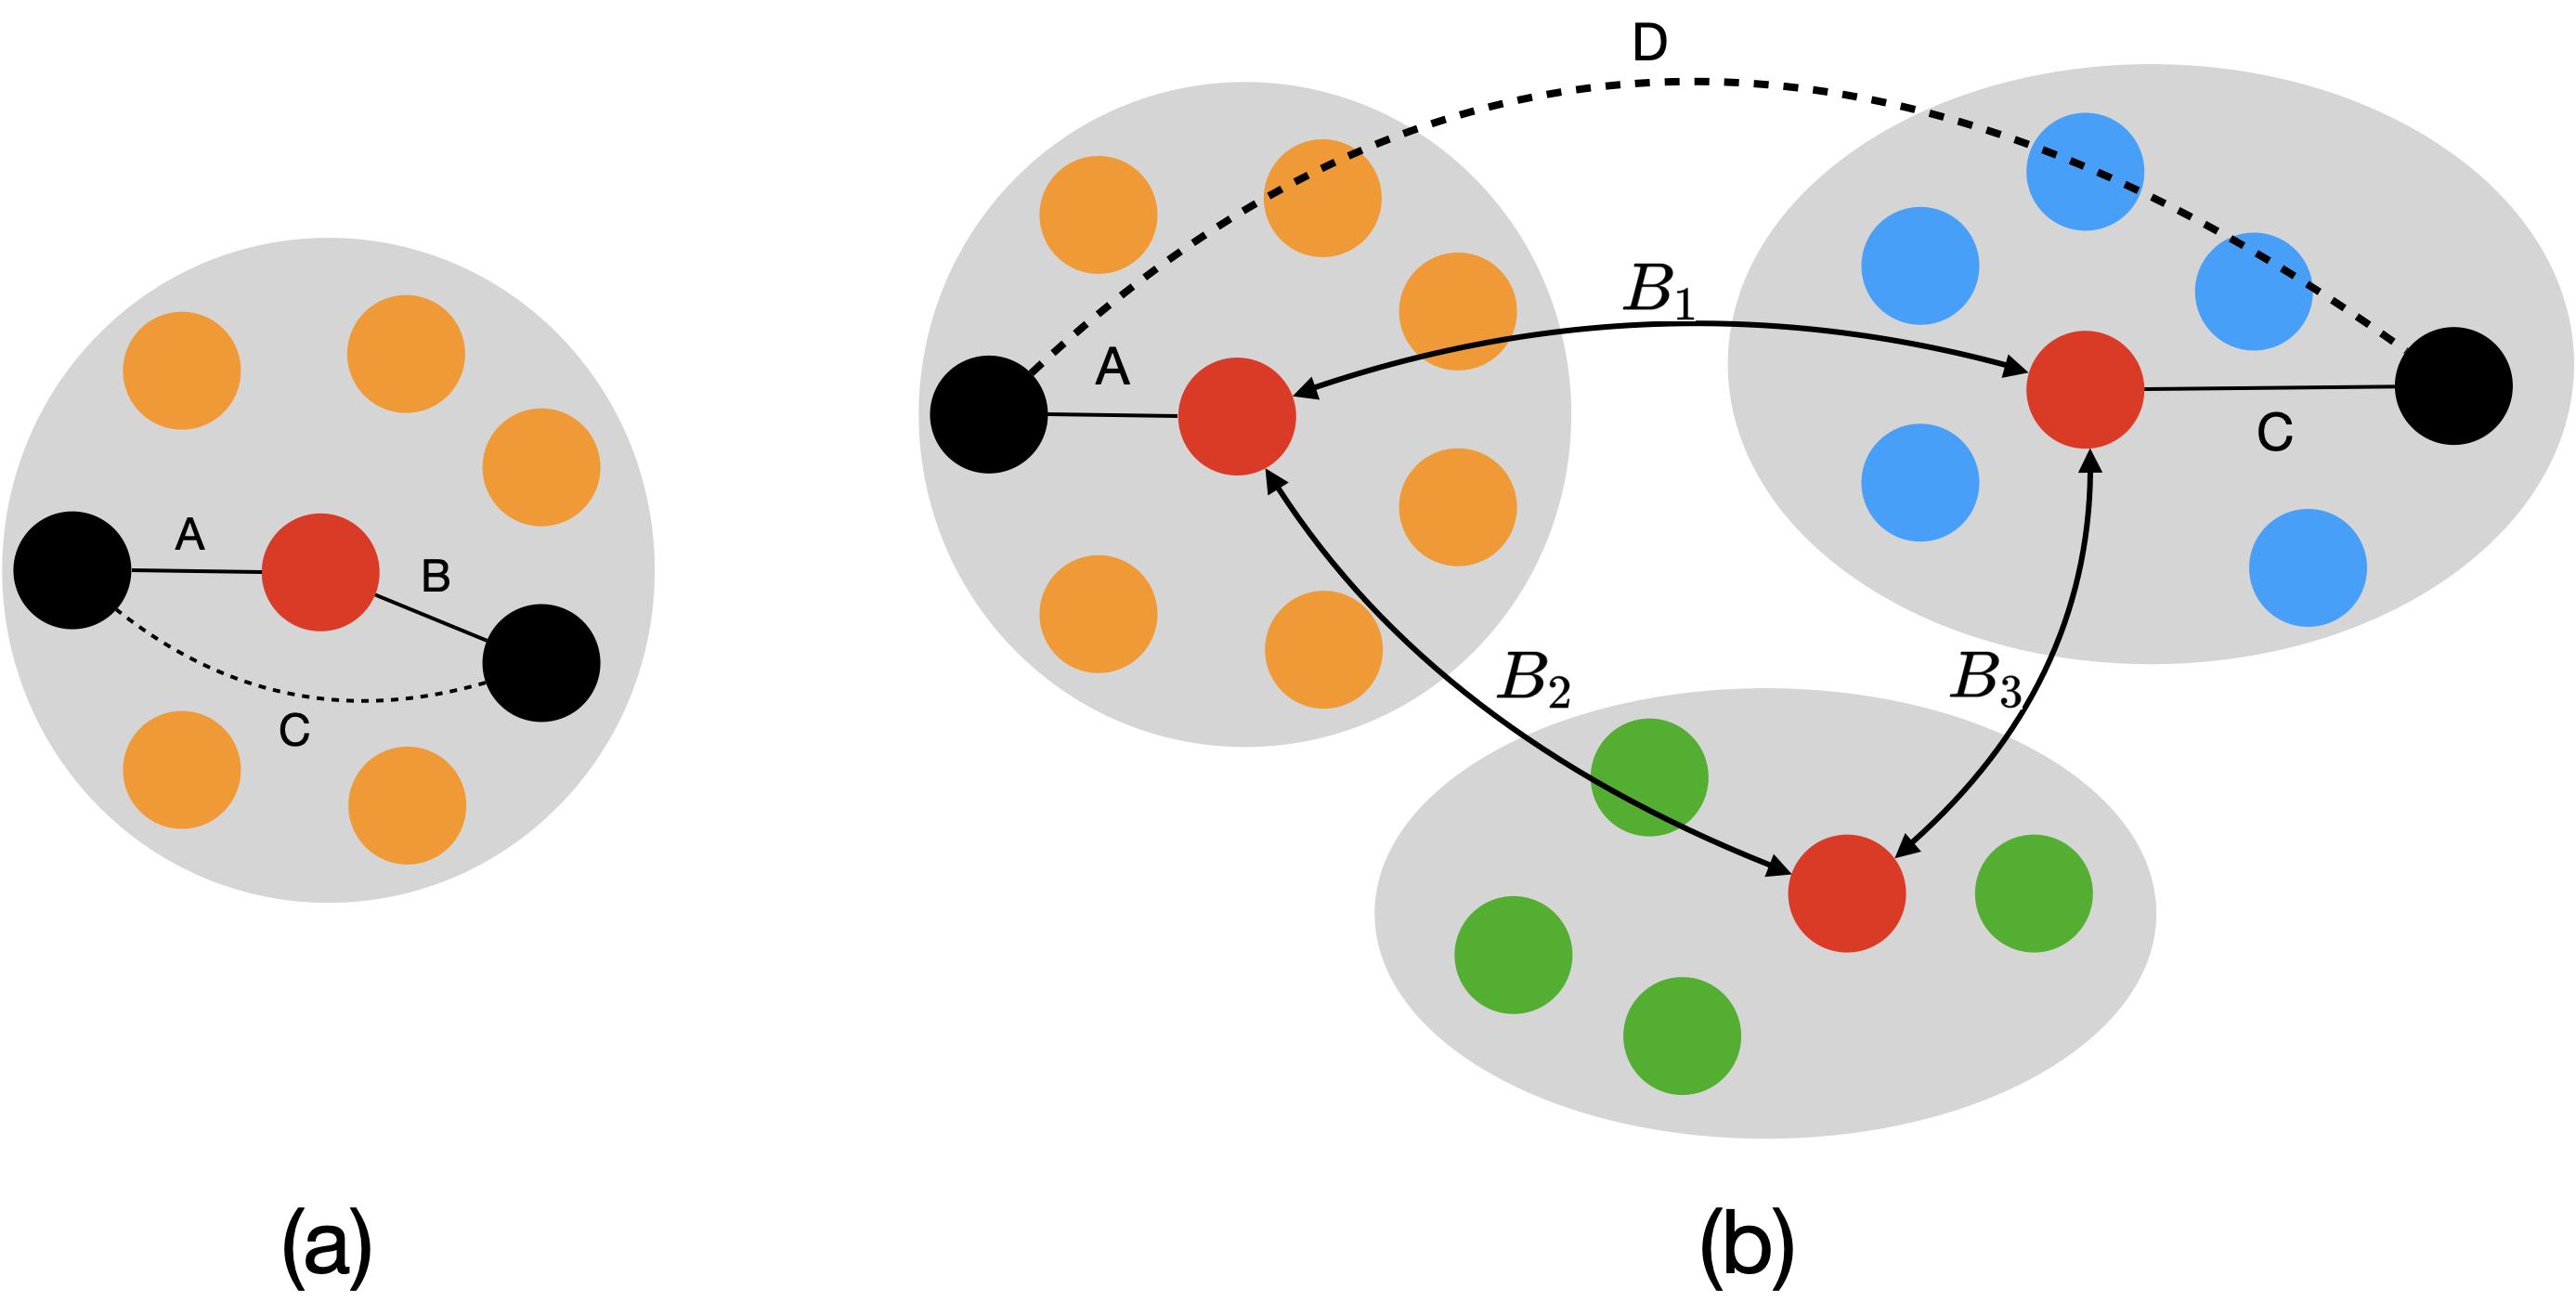
\includegraphics[width=0.4\textwidth]{figures/4-2-query-fram.png}
\caption{Partition Query} 
\label{fig5}
\end{figure}

%
%
Next, we introduce hash region and partition query for further optimization. In our algorithm, hash region technique is a kind of hash table to quickly determine if vertices $s$ and $t$ belong to the same region. During the query process, we first Check if $s$ and $t$ are in the same region using the hash region. If they are, $\text {distance[s][i] + distance[t][i]}$ is used as the upper bound pruning condition. If not, $\text {distance[s][i] + highway[i][j] + distance[t][j] }$ serves as the upper bound. Subsequently, we conduct a simultaneous bidirectional search initiated from both $s$ and $t$ in $G[V \setminus R]$ under the upper bound $\underline{d}_{s,t}$. \par
%

\begin{example}
   Refer to the graph shown in Fig.~\ref{fig5}, black vertices represent the vertices to be queried, and red vertices represent the finalized landmarks. In Fig.~\ref{fig5}(a), after region-based hash determines that $s$ and $t$ belong to the same region, a bidirectional BFS is executed. The process terminates when the distance $C$ exceeds $A + B$, at which $d_{G}(s, t)=A+B$ is confirmed as the shortest distance. In Fig.~\ref{fig5}(b), orange, green, and blue vertices each represent vertices within the same region. After region-based hash determines that $s$ and $t$ do not belong to the same region, a bidirectional BFS is executed. The process terminates once the distance $D$ exceeds $A+\min \{B 1, B 2+B 3\}+C$, establishing $d_{G}(s, t)=A+\min \{B 1, B 2+B 3\}+C$ as the shortest distance. Note that, $B_{1}$, $B_{2}$ and $B_{3}$ can be directly obtained through the highway. 
\end{example}

%
%
\section{Landmark Selection}
\label{sec:landmark_selection}
In this section, we propose an innovative strategy for selecting important vertices, referred to as landmarks, in a graph. This approach seeks to improve upon the traditional method of selecting the top-K vertices with the highest degrees by incorporating a more nuanced iterative regional division process. \par

\begin{algorithm}
\caption{Landmark Selection}
\SetAlgoLined
\DontPrintSemicolon
\KwIn{$G = (V, E);$}
\KwOut{$topk[];$}
\SetKwFunction{FMain}{SelectLandmarks}
\SetKwProg{Fn}{Function}{:}{}
\Fn{\FMain{$Graph \ G$}}{
    $topk[] \leftarrow$\ select $K$ highest degree vertices as landmarks;\;
    \ForEach{landmark $j$ in $topk$}{
        Perform BFS from $j$ to calculate distances;\;
    }
    \ForEach{$i = 0$ \KwTo $V-1$}{
        \If{$i$ not in $topk$}{
            Find the nearest landmark for vertex $i$ and assign to its region\;
        }
    }
    \ForEach{$i = 0$ \KwTo $K-1$}{
        \ForEach{vertex in $regions[i]$}{
            Find MaxDgreeVertex;\;
        }
        $topK[vertex] \leftarrow MaxDgreeVertex$\;
    }
    \Return $topk[];$\
}
\end{algorithm}
%
%
Algorithm 3 describes how our algorithm select landmarks. The strategy enhances efficiency and effectiveness in graph processing tasks. The detailed methodology is as follows: (i) \textbf{Initial Step:} We begin by selecting the top-K vertices with the highest degrees in the graph as the initial set of landmarks. This step serves as the foundation for the subsequent iterative process, providing initial vertices for the refinement of landmark selection. (ii) \textbf{Regional Division Step:} Next, each vertex not already designated as a landmark is assigned to the region associated with the nearest landmark. This division creates a dedicated influence zone for each landmark, simplifying the search space for subsequent queries and thus enhancing query speed. (iii) \textbf{New Landmark Selection Step}: Each region is considered independently, which only considers the connections within the region and ignores the connections across regions. On this basis, we select a vertex with the highest degree within each region as a new landmark to ensure efficiency and accuracy in query operations.\par

Through such strategy, we construct a set of landmarks that not only considers vertex significance but also optimizes spatial locality, significantly speeding up subsequent algorithm queries. The essence of this method lies in its ability to rapidly locate the area relevant to a query, reducing unnecessary search and computation, offering a new pathway for efficient processing of large-scale graph data.\par

It should be noted that due to the Order Independence \cite{ref7} property  of highway cover labeling, there is no need to consider the attribution of a vertex to different landmarks at the same distance. The vertices that are first traversed belong to the region covered by that landmark.\par
%
%
\begin{proof}
    Defind $Order{L_{1}}$ and $Order{L_{2}}$ as two distance labeling orders over landmark $R$. During the label construction process, the BFS conducted from landmark $r$ in $Order{L_{1}}$ and $Order{L_{2}}$ traverses the same set of vertices, resulting the same pruded BFS tree. Thus, Algorithm 1 ensures that $L_{1}(v)=L_{2}(v)$ for every $v \in V \backslash R$.
\end{proof}

%
%
\begin{figure}
\centering
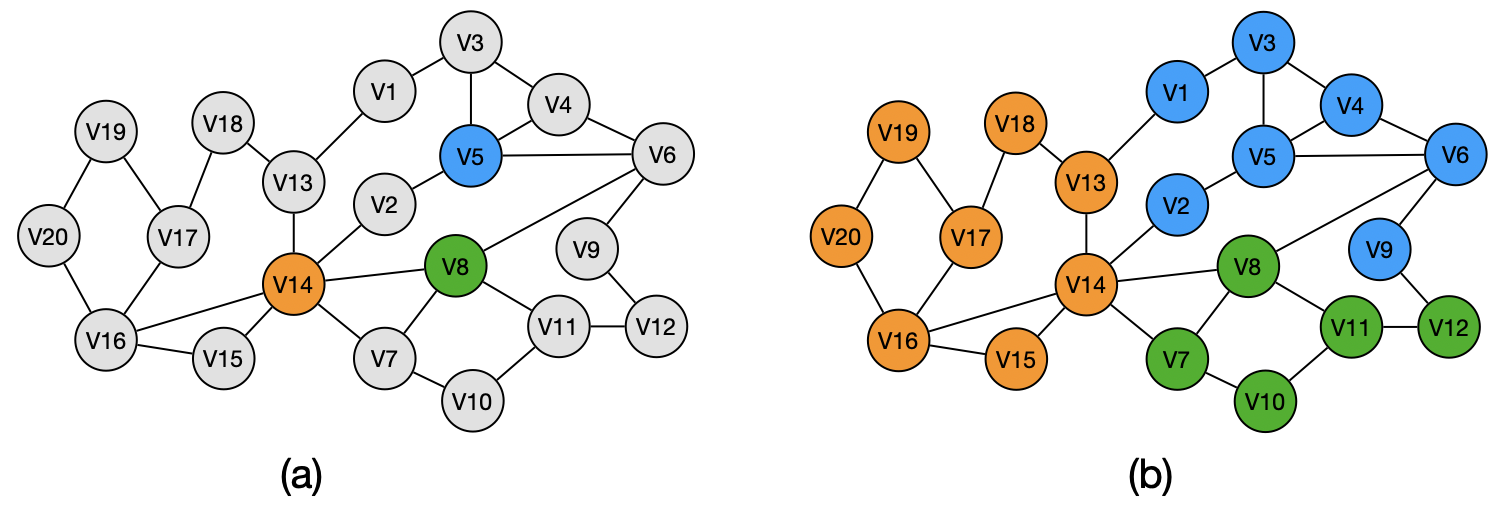
\includegraphics[width=0.5\textwidth]{figures/5-1-landmark.png} 
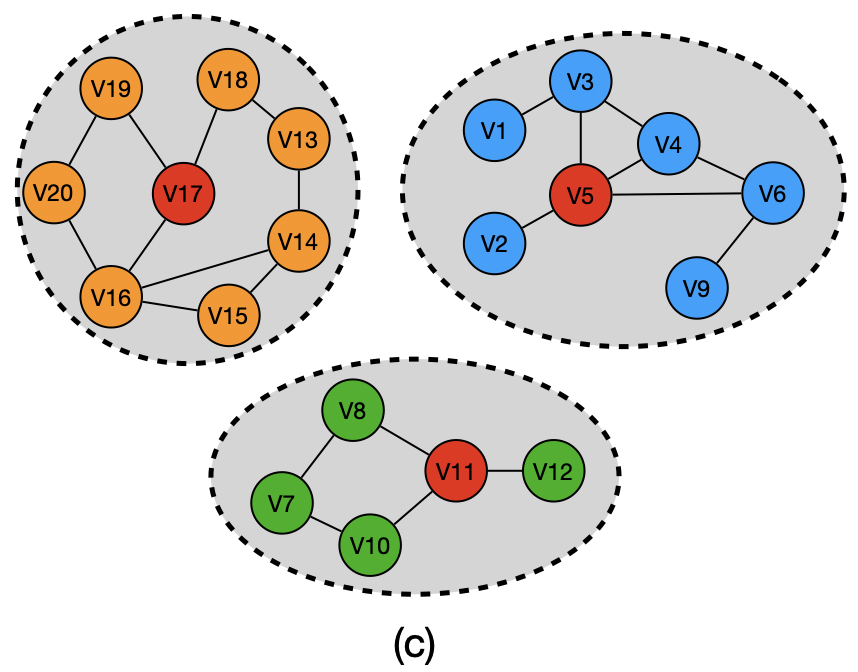
\includegraphics[width=0.35\textwidth]{figures/5-2-lanbdmark.png}
\caption{Landmark Selection.} \label{fig6}
\end{figure}

\begin{example}
    In the network illustrated in Fig.~\ref{fig6}(a), vertices $\left \{ v_{5}, v_{8}, v_{14} \right \} $, which have the highest degrees, are selected as initial landmarks. Starting from each landmark, recording the vertices reachable by each landmark, as shown in Fig.~\ref{fig6}(b). Subsequently, as detailed in Fig.~\ref{fig6}(c), each region is treated independently, with marginalization of vertices, meaning only intra-region edges are counted while inter-region connections are excluded. Within each region, the vertex with the highest degree, vertices $\left \{ v_{5}, v_{11}, v_{17} \right \} $ marked in red, is selected as the final landmark.
\end{example}
%
%
\section{Experiment}
\label{sec:Experiment}
In this section, we present extensive experiments to evaluate our methods. All algorithms were implemented in C++11 using the Standard Template Library (STL) and tested on a server with an Intel Xeon 2.10GHz CPU, 256GB of RAM, and Ubuntu 20.04. The experimental code was written in C++.
\subsection{Datasets}
%
%



\begin{table}[h]
\centering
\caption{Datasets}
\resizebox{.3\textwidth}{!}{ % 调整表格宽度为页面宽度
\begin{tabular}{lcc}
\toprule
\textbf{Network} & \textbf{Vertices $n$} & \textbf{Edges $m$} \\
\midrule
Douban     & 154,909   & 654,324    \\
Amazon     & 334,863   & 1,851,744    \\
DBLP       & 317,980   & 2,099,732  \\
Youtube    & 1,134,890 & 5,975,248  \\
As-skitter & 1,696,415 & 22,190,596 \\
\bottomrule
\end{tabular}
}
\label{tab:datasets}
\end{table}

We use five publicly available real-world networks from the Stanford Network Analysis Project\cite{ref14}. Table \ref{tab:datasets} provides details of these datasets, which we treated as undirected graphs.
\subsection{Query Performance Comparison}

\begin{table}[!htbp]
\caption{Random vertex pair shortest distance batch query}
\label{tab:Performance}
\centering
\renewcommand\arraystretch{1.2}
\resizebox{0.7\linewidth}{!}{
\begin{tabular}{ l c c c c c c c}
    \hline
        Datasets & HL & Naive-KHL & KHL \\
        \hline
        douban & 0.806s & 0.799s & 0.613s \\
        amazon & 5.863s & 5.841s & 4.201s \\
        dblp & 1.96s & 1.791s & 1.538s \\
        youtube & 6.584s & 5.863s & 5.164s \\
        as-skitter & 11.816s & 11.174s & 8.933s \\
        \hline
        \end{tabular}
    }
\end{table}
%
%
To evaluate the average query time, we randomly generate one million vertex pairs from each graph for batch processing of shortest path distance queries. The results are shown in Table \ref{tab:Performance}. Our algorithm KHL denotes a region hash optimization based on the use of a new landmark selection strategy. The Naive-KHL method denotes no region hash optimization. This optimization is described in Section \ref{sec:query_distance}. The HL algorithm used in our experiments is derived from\cite{ref7} which selects the top $k$ highest degree vertices as landmarks without any optimization during the query phase. Experimental validation demonstrated that our algorithm enhances query speed by 20\%-30\% in large networks compared to traditional methods.\par
%
%
\subsection{Overlap rates}
%
%
\begin{figure}
\centering
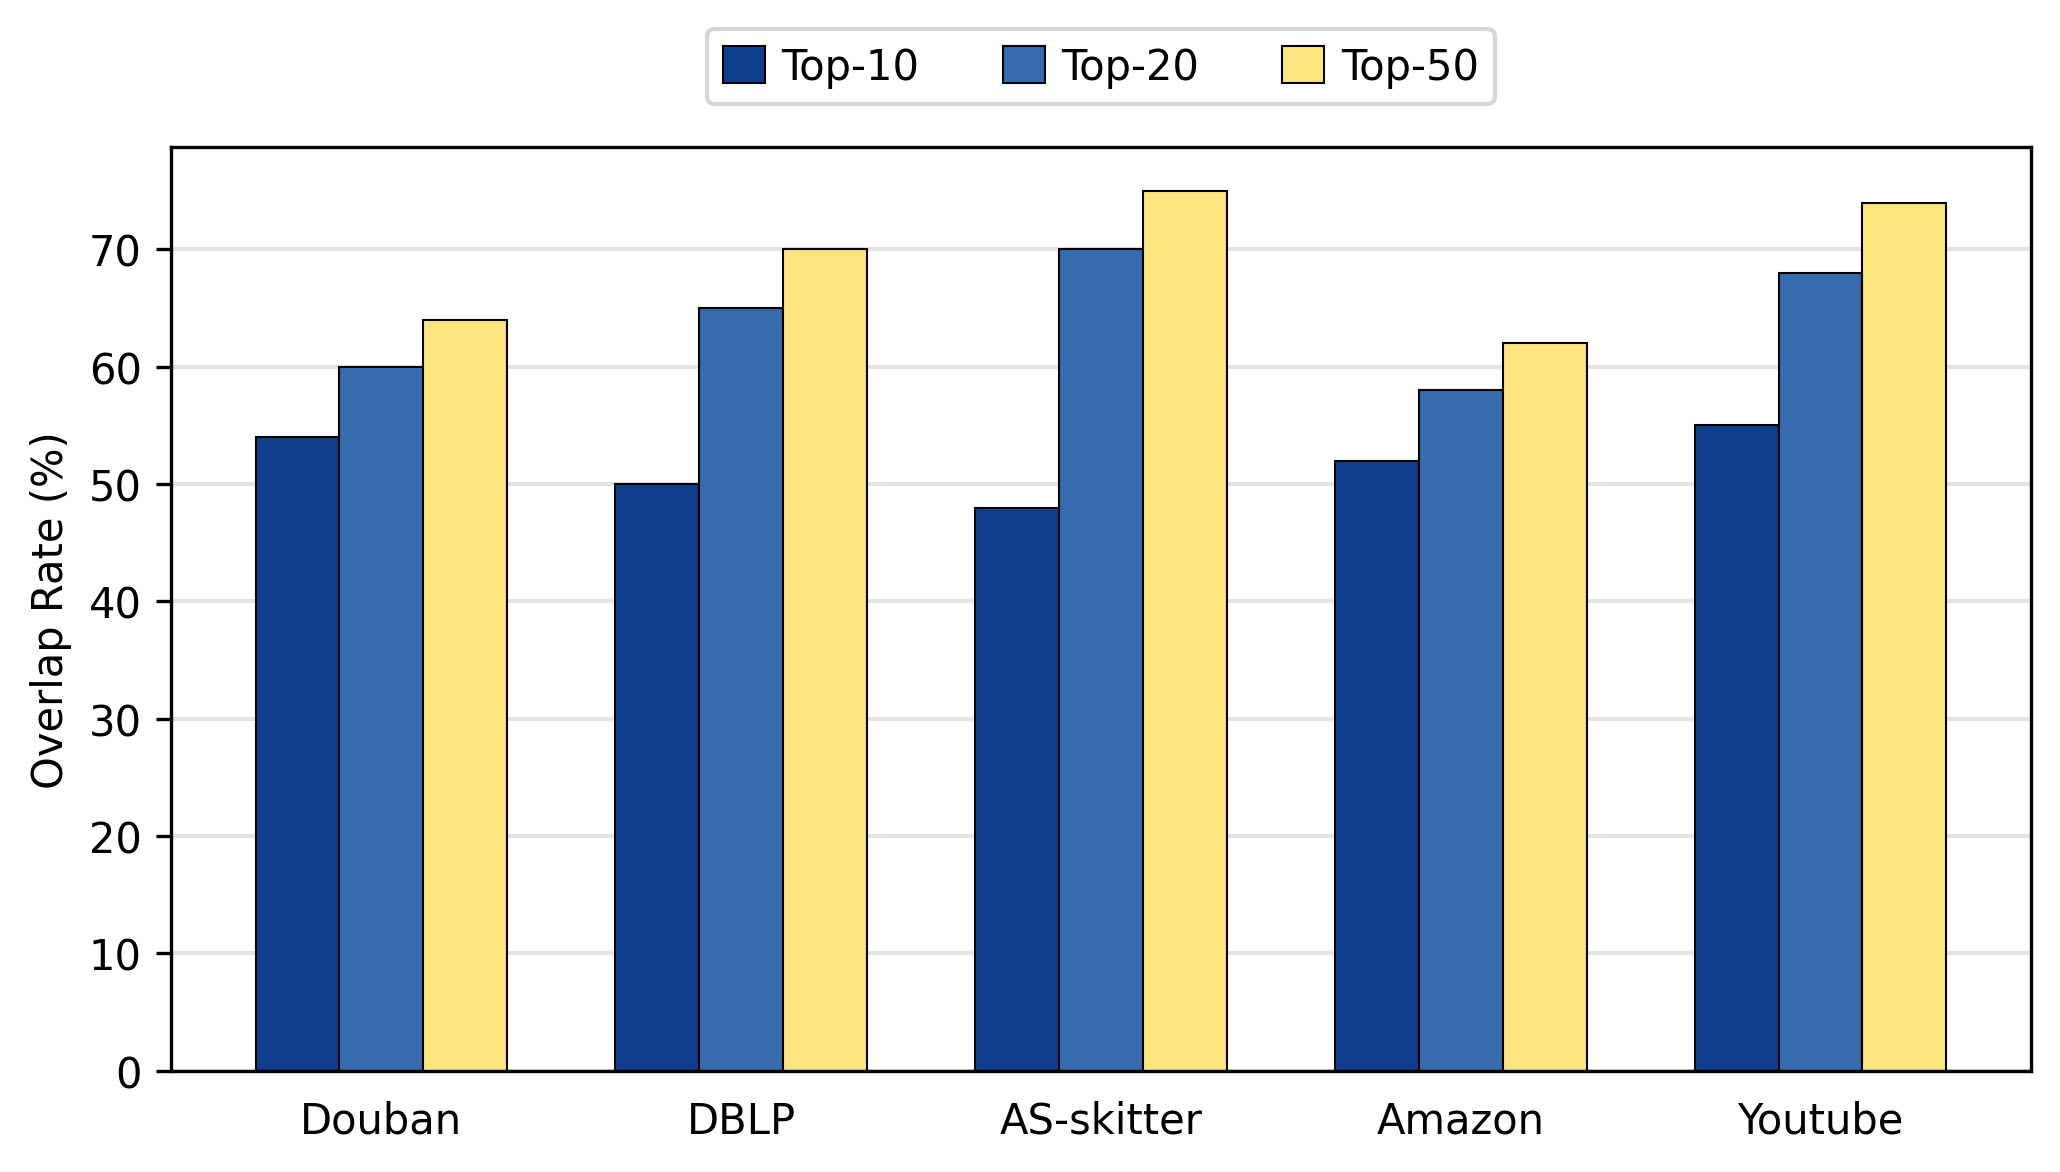
\includegraphics[width=0.5\textwidth]{figures/5-3-overlap_rates.png}
\caption{Overlap rates} 
\label{fig7}
\end{figure}
%
%
We conducted experimental analysis on the selected vertices as landmarks using Top-k degree and Top-k betweenness methods. The horizontal axis represents the dataset, and the vertical axis represents the overlap rate. We compared the overlap rates of selected vertices as landmarks under the conditions of setting the number of landmarks at $10$, $20$, and $50$, respectively. Fig.~\ref{fig7} shows that these two traditional methods have a high overlap rates in the selected landmarks. Due to the properties of degree, vertices near those with a higher degree also tend to have higher degrees, resulting in a clustered arrangement of landmarks. The experiments indicated that the high overlap rate also leads to clustering when landmarks are selected based on betweenness. Thus, ensuring a dispersed distribution of landmarks, which can cover more shortest paths between vertex pairs, is a crucial optimization. Our method ensures zero overlap with the landmarks selected by traditional methods.\par
%
%
\subsection{Performance under Varying Landmarks}
%
%
\begin{figure}
\centering
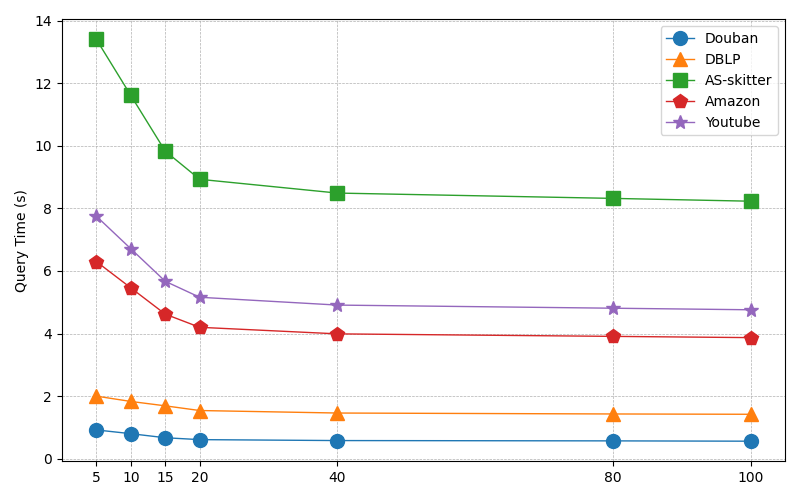
\includegraphics[width=0.5\textwidth]{figures/5-4-varylandmarks.png}
\caption{Performance under Varying Landmarks} 
\label{fig8}
\end{figure}

From Fig.~\ref{fig8}, it can be seen that as the number of landmarks increases, the query speed also increases accordingly. However, adding additional landmarks will result in an increase in preprocessing time and storage space. When the number of landmarks exceeds $20$, the benefits gradually decrease, and further increasing the number of landmarks is difficult to bring effective improvement. Therefore, we consider $20$ landmarks to be an optimal choice.

%
%

\section{Conclusion}
\label{sec:conclusion}
In this study, we propose and implement an innovative landmark selection strategy that improves traditional degree-based methods, significantly enhancing the effectiveness of landmark selection while reducing redundancy and clustering. By integrating partition query and upper-bound pruning optimizations, our algorithm achieved a notable improvement of 20\% to 30\% in query speed and can be applied to datasets comprising tens of millions of records. This research provides new insights and solutions for improving query performance in large-scale graph-structured data, such as graph databases and social networks. Moving forward, we will continue to explore more innovative strategies for optimizing graph databases to meet the growing demands of large-scale graph data processing.

 
\section{Acknowledgments}
According to relevant requirements, this section only makes an academic statement to ensure compliance with research standards and originality requirements. The partial content of the article is only to polish academic writing using the artificial intelligence tool (ChatGPT).
%%
%% The next two lines define the bibliography style to be used, and
%% the bibliography file.
\bibliographystyle{ACM-Reference-Format}
\bibliography{conference-latex-template/sample-base}

\appendix
%%
\end{document}
\endinput
%%
%% End of file `sample-sigconf.tex'.
